\lab{Algorithm}{Pseudorandom Number Generators}{Pseudorandom Number Generators}
\label{Ch:PRNG}

\objective{Learn about the strengths and weaknesses of a few a pseudorandom number generators}

\section*{Random Numbers}

Lotteries, most board games, and statistics need random numbers.
In real life, we roll dice, take balls out of a bag, or spin a wheel.
Computers are, by nature, deterministic, meaning that they do exactly what they are told.
Because of this, random number generation on a computer can be difficult.
We can have a device measure a random process and use the data to generate random numbers, 
But such sampling is often too slow and too expensive for practical use.
Pseudorandom number generators (PRNGs) are a common solution to this problem.
The numbers are not truly random, but they are based on a complex formula that makes them look ``random."
For convenient use, these generateors must also run quickly.
The goal is to have something that is fast and looks random.

There are many different algorithms for developing pseudorandom numbers.
Robert R. Coveyou titled an article ``The generation of random numbers is too important to be left to chance."
There has been much study about different PRNGs.
This lab will cover two of them: Linear Congruiental Generators and The Mersenne Twister.

\section*{Linear Congruential Genterators}

Linear Congruential Generators (LCG) are one of the oldest ways of generating random numbers.
The Generator is defined by the recurrence relation:
$X_{n+1}=(a*X_n + c)$ mod $m$ where

\begin{itemize}
\item $X$ is a sequence of pseudorandom values, and
\item $m$, $0<m$ is the modulus
\item $a$, $0<a<m$ is the multiplier
\item $c$, $0\leq c<m$ is the increment
\item $X_0$, $0\leq X_0 <m$ is the seed
\end{itemize}

each of these are integer constants.

\begin{problem}
Write a LCG that produces an array of pseudorandom numbers between $0.0$ and $1.0$.
Let the arguments be size of the array and let a, c, mod, and seed be optional arguments.
I recommend $a=1103515245$, $c=12345$, $m=2^{31}-1$, and $seed=4329$ as the default values.
\end{problem}

\begin{problem}
Write a LCG that produces an array of pseudorandom numbers of integers between two input arguments.
Do it by calling your algorithm from problem one and multiplying it by the values and casting the array as an int using the .astype() function.
Let the arguments be size of array and the two integers.
Let a, c, mod, and seed continue to be optional arguments.
\end{problem}

One easy way to ``see" if your generator is random is to look at a bitmap of the output.
In python, use the plt.imshow() function to see a bitmap of the array produced by your LCG.
Resize your output to be $512 \times 512$.

\begin{figure}[H]
%\begin{center}

\includegraphics[scale = .4]{PRNG1.jpg}
\caption{
The bitmap with $a=25214903917$, $c=11$, $m=2^{48}$.
There is a clear pattern in the random numbers.}
%\end{center}
\end{figure}

\begin{problem}
For what values of $a$, $c$, and $m$ does your LCG have a visible pattern.
\end{problem}

This method is not rigorous, but there are several other ways to test the randomness of your output.

The length over which your random number generator repeats is called the period.
The period is at most m, but it may be shorter based on the values of a and c.
 
\begin{comment}
According to the Hull-Dobell Theorem (TO DO: find a source), a LCG will have a full period if and only if, 
1. $c$ and $m$ are relatively prime,
2. $a-1$ is divisible by all prime factors of $m$,
3. $a-1$ is a multiple of 4 if $m$ is a multiple of 4

\begin{problem}
Test values of $a$,$c$, and $m$ that fit these requirements. 
\end{problem}
\end{comment}

This algorithm is used as the default random number generator in Java, and C++ and is still used in a wide variety of situations.

\section*{Mersenne Twister}

\begin{comment}
(TO DO: decide how much of  this we want to keep) All numbers can be represented in bits as a base two number.
Computers are optimized to work with numbers in that manner.
The operators XOR, OR, and AND work on the bit representation of two numbers.

AND - if both numbers have a 1 in the ith place then the ith place is 1.
Otherwise the ith place is 0.

OR - if one or both numbers have a 1 in the ith place then the ith place is 1.
Otherwise the ith place is 0.

XOR - if only one of the two numbers has a 1 in the ith place then the ith place is 1.
If both or neither of the numbers has a 1 in the ith place, the ith place is 0.

In addition you can shift the bitwise number over a number of values.
For example, shifting 10100 to the right by one yields 1010 and shifting it to the left by one yields 101000.
This is really just division and multiplication by 2.
This can be done by $\ll$ and $\gg$ in python. 
\end{comment}

The Mersenne twister PRNG does a series of bitwise operations to generate random numbers.
The Random class in python uses the Mersenne twister algorithm. 

\begin{problem}
Look at the bitmap of output of sp.rand(512,512).
Can you see any patterns?
\end{problem}

\section*{Randomness Tests}

There have been statistical tests devised for measuring the quality of a random number generator. One is these is the overlapping permutations test. Analyze sequences of five consecutive random numbers. The 120 possible orderings should occur with statistically equal probability.

\begin{problem}
Use the overlappng permutations test to see how random python's random number generator is compared to the LCG you wrote in problem 1.
\end{problem}

\section*{Blackjack}

\begin{figure}[H]
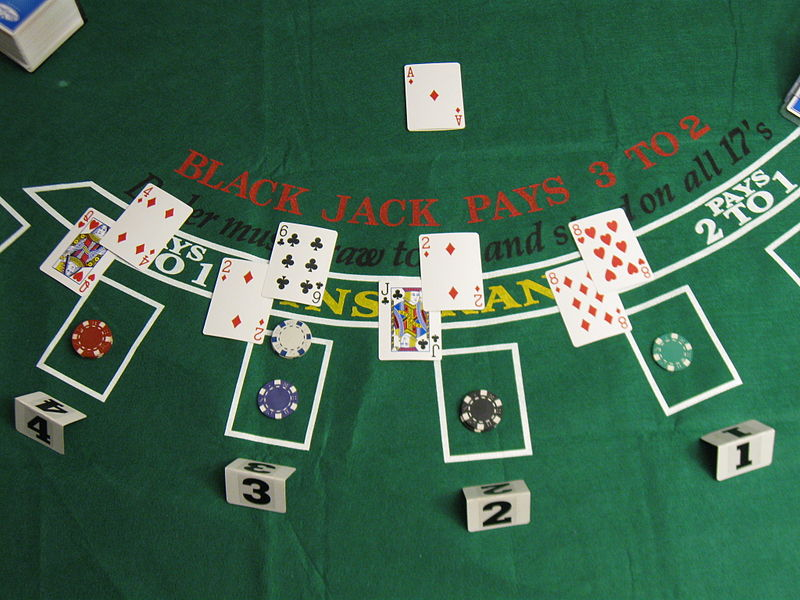
\includegraphics[scale = .9]{Blackjack_game_1.jpg}
\caption{Initial Round of a BlackJack Game}
\end{figure}

Black Jack is a card game that involves the use of randomness.
The game is simple.
The dealer deals the player and himself each two cards.
He flips over his first card so that the player can see it.
The player has to choose to take another card ("hit") or not ("stand").
If the player hits he gets another card and again has the choice to hit or stand.

The goal is to get your hand to be at or as close to 21 without going over.
Face cards are worth 10 points.
Aces can count either as 11 or 1.
The value of all other cards are equal to number on the card.

Once the player has decided to stand the dealer flips over his second card and deals himself cards until his hand value is 17 or greater. 

If the player value goes above 21 he automatically loses.
If his value is 21 and below and dealer has above 21 then the player wins.
If they both have 21 or under than the player with the hand of highest value wins.
If both hands have the same value, the game is a tie.

\section*{Shuffling Algorithms}

One use of Pseudorandom Number Generators (PRNGs) is to shuffle cards.
The main goal of these algorithms is that the card order be random--so that no single player has an advantage based on order.
Often, as strange as it may seem, online gambling sites will post their shuffling algorithms online.
The only things they do not post are their seed values.
Often the time in milliseconds from midnight is used as the seed value.

John von Neumann said ``Anyone who considers arithmetical methods of producing random digits is, of course, in a state of sin."
As seen in the last lab, weak PRNGs are periodic and are predictable once a few outputs are known.
This lab will have you break blackjack based on a weak PRNG.

\section*{Cracking Blackjack}
For these next problems you will need three files that are provided with this lab: Black.py, BlackEasy.py, and bjHelp.py.
Black.py and BlackEasy.py are are programs that run games of Blackjack that use a Linear Congruentail Generator (LCG) to shuffle the cards.
They generate 52 random numbers and then the argsort of those numbers is the order of the cards.
The parameters for BlackEasy.py are a$=2521$, c$=13$, mod$=2^{16}$.
For Black.py they are a$=25214903917$, c$=11$, mod$=2^{48}$.
In order to play them type \li{python <<filename>> <<numberofgames>>} in your command line.
They are both seeded initially by the time.

bjHelp.py contains two functions that will help you "predict" the cards:
SuffleHack(n,a,c,mod,seed) gives the first $n$ card shuffles given the parameters for a LCG.
The shuffles are represented by numbers.
Hacker(Stats,['card','card','card']) Stats is the output of SuffleHack and takes a list of 3 cards (see below).
It prints all shuffles as a list of cards in Stats that have the same first three cards as the inputted list.

The trick to being able to "predict" the cards is to find the initial seed value.

Cards- A, 2-10, J, Q, or K combined with heart, diamond, club, or spade in single quotes.
Examples: '6diamond', 'Kclub'.

\begin{warn}
Both BlackEasy.py and Black.py use functions that are incompatible with ipython. They need to run \li{python Black.py} in command line.
\end{warn}



\begin{problem}
Play 10 games of BlackEasy.py and by the 5th game be able to predict the cards.
You can write your own functions or use the ones in bjHelp.py.
You will want to open two command prompts, one to play the game and one to predict the cards. 
\end{problem}

Not too hard.
That is because there is only $2^{16}$ seed values.
This next one you will have to look at more hands until you can find out the initial seed value.

\begin{problem}
Play 20 games of Black.py and by the 15th game be able to predict the cards.
\end{problem}
